\section{Arjun Yuda Firwanda}
\subsection{Soal 1}
Isi jawaban soal ke-1

Kalau mau dibikin paragrap \textbf{cukup enter aja}, tidak usah pakai \verb|par| dsb

%\subsection{Soal 2}
%Isi jawaban soal ke-2

%\subsection{Soal 3}
%Isi jawaban soal ke-3

\section{Dwi Yulianingsih}
\subsection{Soal 1}
Isi jawaban soal ke-1

Kalau mau dibikin paragrap \textbf{cukup enter aja}, tidak usah pakai \verb|par| dsb

%\subsection{Soal 2}
%Isi jawaban soal ke-2

%\subsection{Soal 3}
%Isi jawaban soal ke-3

\section{Harun Ar-Rasyid}
\subsection{Soal 1}
Isi jawaban soal ke-1

Kalau mau dibikin paragrap \textbf{cukup enter aja}, tidak usah pakai \verb|par| dsb

%\subsection{Soal 2}
%Isi jawaban soal ke-2

%\subsection{Soal 3}
%Isi jawaban soal ke-3

\section{Sri Rahayu}
\subsection{Soal 1}
Isi jawaban soal ke-1

Kalau mau dibikin paragrap \textbf{cukup enter aja}, tidak usah pakai \verb|par| dsb

%\subsection{Soal 2}
%Isi jawaban soal ke-2

%\subsection{Soal 3}
%Isi jawaban soal ke-3

\section{Doli Jonviter}
\subsection{Soal 1}
Isi jawaban soal ke-1

Kalau mau dibikin paragrap \textbf{cukup enter aja}, tidak usah pakai \verb|par| dsb

%\subsection{Soal 2}
%Isi jawaban soal ke-2

%\subsection{Soal 3}
%Isi jawaban soal ke-3

\section{Rahmatul Ridha}
\subsection{Soal 1}
\subsection{Instalasi Anaconda}
\begin{itemize}
\item Instalasi Anaconda
Berikut adalah langkah-langkah cara menginstal Anaconda di Windows:
\begin{enumerate}
\item Download installer anaconda terbaru, seperti pada gambar \ref{downloadanaconda}. Kalian dapat memilih versi 2 atau 3, dengan versi Anaconda berapa.
\begin{figure}[ht] \centerline{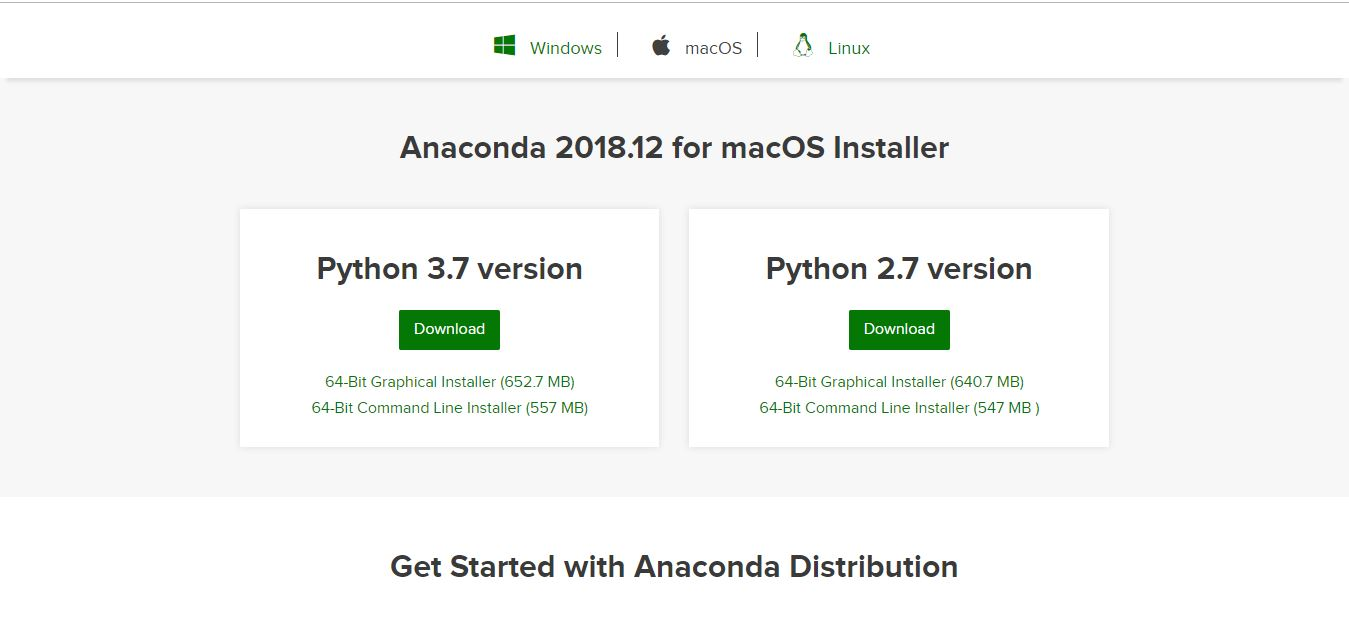
\includegraphics[width=0.70\textwidth]{figures/1/1144124/DownloadAnaconda.JPG}}
	\caption{Download Anaconda}
	\label{downloadanaconda}
\end{figure}
	
\item Setelah selesai mendownload, klik 2 kali pada installer Anaconda.
\item Kemudian akan tampil seperti gambar \ref{gambar1}, lalu klik next.
\begin{figure}[ht]
	\centerline{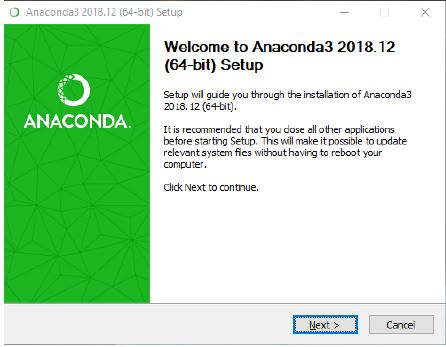
\includegraphics[width=0.70\textwidth]{figures/1/1144124/a.JPG}}
	\caption{Proses 1 }
	\label{gambar1}
\end{figure}

\item Setelah itu read lisensi dan klik `I Agree' seperti pada gambar \ref{gambar2}.
\begin{figure}[ht]
	\centerline{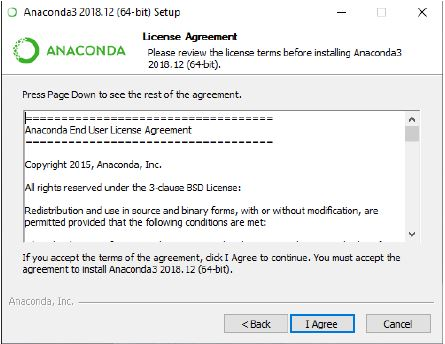
\includegraphics[width=0.70\textwidth]{figures/1/1144124/b.JPG}}
	\caption{proses 2 }
	\label{gambar2}
\end{figure}

\item Selanjutnya ada pilihan untuk menginstallnya, yaitu `just me' atau `all users'. Lalu klik next seperti pada gambar \ref{gambar3}.
\begin{figure}[ht]
	\centerline{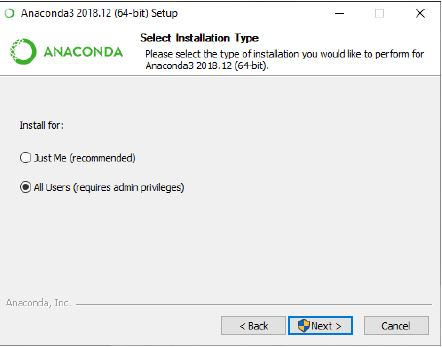
\includegraphics[width=0.70\textwidth]{figures/1/1144124/c.JPG}}
	\caption{Proses 3 }
	\label{gambar3}
\end{figure}

\item Kemudian pilih okasi yang diinginkan, lalu klik next seperti pada gambar \ref{gambar4}.
\begin{figure}[ht]
	\centerline{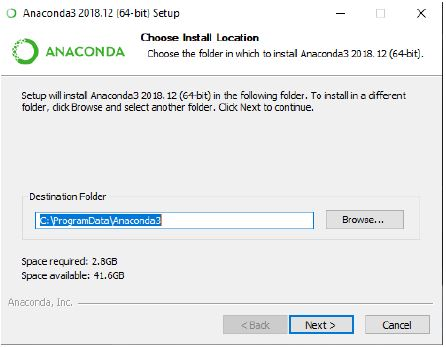
\includegraphics[width=0.70\textwidth]{figures/1/1144124/d.JPG}}
	\caption{Proses 4 }
	\label{gambar4}
\end{figure}

\item Pilih ‘add anaconda to PATH’ atau tidak. Disini kalian memilih apakah akan mendaftarkan Anaconda sebagai default Python 3.7. kacuali kalian berencana menginstal dan menjalankan beberapa versi Anaconda, atau beberapa versi Python, biarkan default dan biarkan kotaknya dicentang. Kemudian klik tombol Install. Jika kalian ingin melihat packages Anaconda yang sedang dipasang, klik Show Details seperti pada gambar \ref{gambar5}.
\begin{figure}[ht]
	\centerline{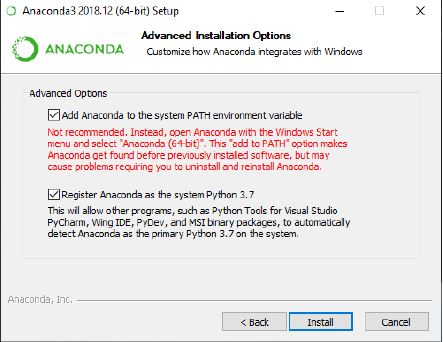
\includegraphics[width=0.70\textwidth]{figures/1/1144124/e.JPG}}
	\caption{Proses 5 }
	\label{gambar5}
\end{figure}

\item Jika instalasi selesai, kemudian klik next seperti pada gambar \ref{gambar6}.
\begin{figure}[ht]
	\centerline{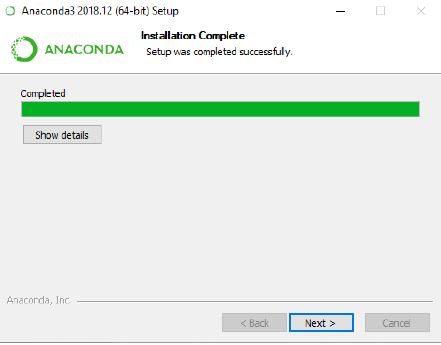
\includegraphics[width=0.70\textwidth]{figures/1/1144124/f.JPG}}
	\caption{Proses 6 }
	\label{gambar6}
\end{figure}

\item Jika packages telah selesai diinstall, maka aka nada perintah untuk menginstall VS Code, lalu klik tombol Install Microsoft VS Code seperti pada gambar \ref{gambar7}.
\begin{figure}[ht]
	\centerline{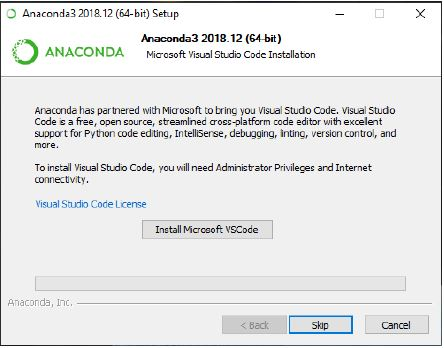
\includegraphics[width=0.70\textwidth]{figures/1/1144124/g.JPG}}
	\caption{Proses 7}
	\label{gambar7}
\end{figure}

\item Setelah instalasi selesai, maka akan terlihat kotal dialog `Thanks for Installing Anaconda3'. Lalu klik Finish seperti pada gambar \ref{gambar8}.
\begin{figure}[ht]
	\centerline{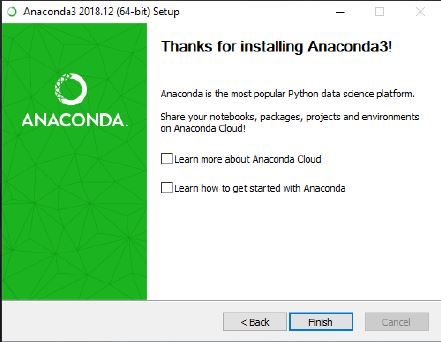
\includegraphics[width=0.70\textwidth]{figures/1/1144124/h.JPG}}
	\caption{Proses 8}
	\label{gambar8}
\end{figure}
	    \end{enumerate}
\end{itemize}

\section{Tomy Prawoto}
\subsection{Soal 1}
Isi jawaban soal ke-1

Kalau mau dibikin paragrap \textbf{cukup enter aja}, tidak usah pakai \verb|par| dsb

%\subsection{Soal 2}
%Isi jawaban soal ke-2

%\subsection{Soal 3}
%Isi jawaban soal ke-3
